

\tikzset{every picture/.style={line width=0.75pt}} %set default line width to 0.75pt        
\begin{figure}[htbp]
    \centering
    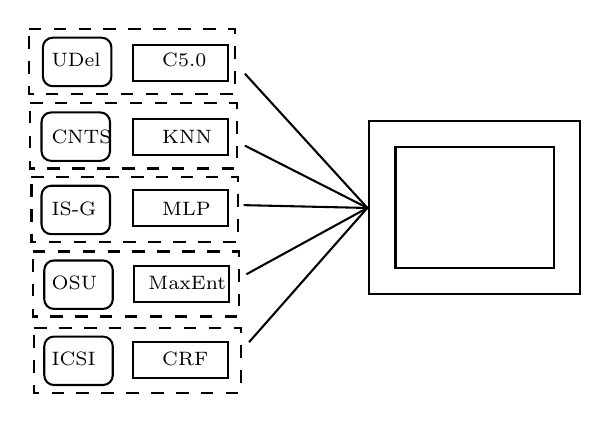
\begin{tikzpicture}[x=0.50pt,y=0.50pt,yscale=-1,xscale=1]
%uncomment if require: \path (0,300); %set diagram left start at 0, and has height of 300

%Rounded Rect [id:dp11696032525693911] 
\draw   (6,30) .. controls (6,26.13) and (9.13,23) .. (13,23) -- (48.5,23) .. controls (52.37,23) and (55.5,26.13) .. (55.5,30) -- (55.5,51) .. controls (55.5,54.87) and (52.37,58) .. (48.5,58) -- (13,58) .. controls (9.13,58) and (6,54.87) .. (6,51) -- cycle ;
%Rounded Rect [id:dp07799259931950897] 
\draw   (5,84) .. controls (5,80.13) and (8.13,77) .. (12,77) -- (47.5,77) .. controls (51.37,77) and (54.5,80.13) .. (54.5,84) -- (54.5,105) .. controls (54.5,108.87) and (51.37,112) .. (47.5,112) -- (12,112) .. controls (8.13,112) and (5,108.87) .. (5,105) -- cycle ;
%Rounded Rect [id:dp6057157286378516] 
\draw   (5,137) .. controls (5,133.13) and (8.13,130) .. (12,130) -- (47.5,130) .. controls (51.37,130) and (54.5,133.13) .. (54.5,137) -- (54.5,158) .. controls (54.5,161.87) and (51.37,165) .. (47.5,165) -- (12,165) .. controls (8.13,165) and (5,161.87) .. (5,158) -- cycle ;
%Rounded Rect [id:dp05149661187443377] 
\draw   (7,191) .. controls (7,187.13) and (10.13,184) .. (14,184) -- (49.5,184) .. controls (53.37,184) and (56.5,187.13) .. (56.5,191) -- (56.5,212) .. controls (56.5,215.87) and (53.37,219) .. (49.5,219) -- (14,219) .. controls (10.13,219) and (7,215.87) .. (7,212) -- cycle ;
%Rounded Rect [id:dp5106057202150704] 
\draw   (7,246) .. controls (7,242.13) and (10.13,239) .. (14,239) -- (49.5,239) .. controls (53.37,239) and (56.5,242.13) .. (56.5,246) -- (56.5,267) .. controls (56.5,270.87) and (53.37,274) .. (49.5,274) -- (14,274) .. controls (10.13,274) and (7,270.87) .. (7,267) -- cycle ;
%Shape: Rectangle [id:dp4932792416812033] 
\draw   (71,28) -- (139.5,28) -- (139.5,54) -- (71,54) -- cycle ;
%Shape: Rectangle [id:dp18275608668220578] 
\draw   (71,82) -- (139.5,82) -- (139.5,108) -- (71,108) -- cycle ;
%Shape: Rectangle [id:dp49550112521417855] 
\draw   (71,133) -- (139.5,133) -- (139.5,159) -- (71,159) -- cycle ;
%Shape: Rectangle [id:dp7299903908595833] 
\draw   (72,188) -- (140.5,188) -- (140.5,214) -- (72,214) -- cycle ;
%Shape: Rectangle [id:dp29994453006627353] 
\draw   (71,243) -- (139.5,243) -- (139.5,269) -- (71,269) -- cycle ;
%Shape: Frame [id:dp0788278471216437] 
\draw   (242,83) -- (394,83) -- (394,208.5) -- (242,208.5) -- cycle(375.18,101.83) -- (260.83,101.83) -- (260.83,189.68) -- (375.18,189.68) -- cycle ;
%Straight Lines [id:da17320760077273079] 
\draw    (152,49) -- (240.5,146) ;
%Straight Lines [id:da17575985418730822] 
\draw    (152,101) -- (240.5,146) ;
%Straight Lines [id:da30612580255952593] 
\draw    (151,144) -- (238.5,146) ;
%Straight Lines [id:da8325128920363636] 
\draw    (153,194) -- (240.5,146) ;
%Straight Lines [id:da9535817232752342] 
\draw    (155,243) -- (240.5,146) ;
%Shape: Rectangle [id:dp03213107417825167] 
\draw  [dash pattern={on 4.5pt off 4.5pt}] (-4.25,16.5) -- (145,16.5) -- (145,63.5) -- (-4.25,63.5) -- cycle ;
%Shape: Rectangle [id:dp5683744790831955] 
\draw  [dash pattern={on 4.5pt off 4.5pt}] (-3.25,70.5) -- (146,70.5) -- (146,117.5) -- (-3.25,117.5) -- cycle ;
%Shape: Rectangle [id:dp09403085065069972] 
\draw  [dash pattern={on 4.5pt off 4.5pt}] (-2.25,123.5) -- (147,123.5) -- (147,170.5) -- (-2.25,170.5) -- cycle ;
%Shape: Rectangle [id:dp8830923797784842] 
\draw  [dash pattern={on 4.5pt off 4.5pt}] (-1.25,177.5) -- (148,177.5) -- (148,224.5) -- (-1.25,224.5) -- cycle ;
%Shape: Rectangle [id:dp5129842925423971] 
\draw  [dash pattern={on 4.5pt off 4.5pt}] (-0.25,232.5) -- (149,232.5) -- (149,279.5) -- (-0.25,279.5) -- cycle ;

% Text Node
\draw (10,32) node [anchor=north west][inner sep=0.75pt]   [align=left] {{\scriptsize \modname{UDel}}};
% Text Node
\draw (10,88) node [anchor=north west][inner sep=0.75pt]  [font=\scriptsize] [align=left] {\modname{CNTS}};
% Text Node
\draw (10,140) node [anchor=north west][inner sep=0.75pt]  [font=\scriptsize] [align=left] {\modname{IS-G}};
% Text Node
\draw (10,193) node [anchor=north west][inner sep=0.75pt]  [font=\scriptsize] [align=left] {\modname{OSU}};
% Text Node
\draw (10,248) node [anchor=north west][inner sep=0.75pt]  [font=\scriptsize] [align=left] {\modname{ICSI}};
% Text Node
\draw (90,32) node [anchor=north west][inner sep=0.75pt]  [font=\scriptsize] [align=left] {\method{C5.0}};
% Text Node
\draw (90,88) node [anchor=north west][inner sep=0.75pt]  [font=\scriptsize] [align=left] {\method{KNN}};
% Text Node
\draw (90,140) node [anchor=north west][inner sep=0.75pt]  [font=\scriptsize] [align=left] {\method{MLP}};
% Text Node
\draw (80,193) node [anchor=north west][inner sep=0.75pt]  [font=\scriptsize] [align=left] {\method{MaxEnt}};
% Text Node
\draw (90,248) node [anchor=north west][inner sep=0.75pt]  [font=\scriptsize] [align=left] {\method{CRF}};
% Text Node
\draw (280,111) node [anchor=north west][inner sep=0.75pt]  [font=\scriptsize] [align=left] {\msrcor};
% Text Node
\draw (280,140) node [anchor=north west][inner sep=0.75pt]  [font=\scriptsize] [align=left] {\negcor};
% Text Node
\draw (280,168) node [anchor=north west][inner sep=0.75pt]  [font=\scriptsize] [align=left] {\wsj};


\end{tikzpicture} 

    
    \caption[Feature sets and ML methods.]{The feature sets and the ML methods of the five GREC algorithms used to train classifiers on the three corpora.} 
    \label{fig:algoscheme}
\end{figure}
